\documentclass[12pt]{beamer}
%\usepackage{amsmath, comment, amsthm, amssymb, amsfonts, multicol,  graphicx, caption, subcaption, multirow}
\usepackage{algpseudocode}
\usepackage{hyperref}
\graphicspath{ {../Report/Pictures/} }
\usetheme{Boadilla}
\title{Parallel A* Project}
\subtitle{System And Device Programming}
\author{Lorenzo Ippolito, Fabio Mirto, Mattia Rosso}
\institute{Politecnico di Torino}
\date{\today}
\AtBeginSection[]{
    \begin{frame}<beamer>
        \frametitle{Outline}
        \begin{columns}[T]
            \begin{column}{.45\textwidth}
                \tableofcontents[currentsection,sections=1-6,hideallsubsections]
            \end{column}
            \begin{column}{.45\textwidth}
                \tableofcontents[currentsection,sections=7-11,hideallsubsections]
            \end{column}
        \end{columns}
    \end{frame}
}
%\usetheme{lucid}
\begin{document}
	\begin{frame}
		\titlepage
	\end{frame}
	\begin{frame}[allowframebreaks]{Outline}
		\tableofcontents
	\end{frame}
	%% %%%%%%%%%%%%%%%%%%%%%%%%%% %%
	%% CHAPTER 1: A* INTRODUCTION %%
	%% %%%%%%%%%%%%%%%%%%%%%%%%%% %%
	\section{Introduction: about the A* algorithm}
	\subsection{Problem definition}
	\begin{frame}{\secname}
		\framesubtitle{\subsecname}
		\begin{itemize}
			\item A* is a graph-traversal and path-search algorithm used in many contexts of computer science and 
			      not only
			\item It can be considered as a general case of the Dijkstra algorithm
			\item It is a Greedy-best-first-search algorithm that uses an heuristic function to guide
				  itself
		\end{itemize}
	\end{frame}
	\begin{frame}{\secname}
		\framesubtitle{\subsecname}
		What it does is combining:
		\begin{itemize}
			\item \textbf{Dijkstra approach}: favoring nodes closed to the starting point(source)
			\item \textbf{Greedy-best-first-search approach}: favoring nodes closed to the final point(destination)
		\end{itemize}
	\end{frame}
	\begin{frame}{\secname}
		\framesubtitle{\subsecname}
		According to the standard terminology:
		\begin{itemize}
			\item $g(n)$: exact cost of moving from source to n
			\item $h(n)$: heuristic estimated cost of moving from a node n(source included) to the destination
			\item $f(n) = g(n) + h(n)$: in this way we are able to combine the actual cost with the estimated one
		\end{itemize}
		At each iteration the node $n$ that has the minimum $f(n)$ is examinated(expanded).
	\end{frame}
	\subsection{Heuristic design}
	\begin{frame}{\secname}
		\framesubtitle{\subsecname: properties}
		The heurstic function represents the acutal core of the A* algorithm. It is a prior-knowledge that
		we have about the cost of the path from every node (source included) to the destination. The properties
		of an heuristic function are:
		\begin{block}{Heuristic function properties}
			\begin{itemize}
			\item 	Admissibility: $h(n) < cost(n, dest) \;\forall n \in V$
			\item 	Consistency: $h(x) \le cost(x, y) + h(y) \; \forall (x, y) \in E$  
			\end{itemize}
		\end{block}
	\end{frame}
	\begin{frame}{\secname}
		\framesubtitle{\subsecname: corner cases}
		Three relevant situations are:
		\begin{itemize}
			\item \textbf{Dijkstra}: if $h(n)=0$ for every node in the graph.
			\item \textbf{Ideal heuristic}: if $h(n)$ is exactly equal to the cost of moving from $n$ to
				  the destination.
			\item \textbf{Full greedy-best-first search}: if $h(n) \gg g(n)$ than only $h(n)$ plays a role.
		\end{itemize}
	\end{frame}
	%% %%%%%%%%%%%%%%%%%%%%%%%%% %%
	%% CHAPTER 2: A* APPLICATION %%
	%% %%%%%%%%%%%%%%%%%%%%%%%%% %%
	\section{A* project application}
	\subsection{Geographical pathfinding}
	\begin{frame}{\secname}
		\framesubtitle{\subsecname}
		We will work with a weighted oriented graph $G$ that is made of nodes $n \in V$ that represents
		road-realated points of interest and edges $(x,y) \in E$ that represent unidirectional connections between these points.
		Each edge $(x, y)$ is associated to a weight that is the great-circle distance between $x$ and $y$ measured
		in meters.
	\end{frame}
	\subsection{Problem-specific heuristic function}
	\begin{frame}{\secname}
		\frametitle{2. A* project application}
		\framesubtitle{The great-circle distance}
		We will apply the Haversine formula to compute the distance from node $(\phi_1,\lambda_1)$
		to node $(\phi_1,\lambda_1)$ where $\phi$ is the latitude and $\lambda$ is the longitude:
		
		\begin{block}{Haversine Formula}
			\begin{center}
				$d = R \cdot c$\\
				$c = 2 \cdot atan2(\sqrt{a},\sqrt{1-a})$\\
				$a = sin^2\Big({\frac{\Delta \phi}{2}}\Big) + cos(\phi_1) \cdot cos(\phi_2) \cdot sin^2\Big({\frac{\Delta \lambda}{2}}\Big)$
				\\$R=6.371km$
			\end{center}
		\end{block}
	\end{frame}
	%% %%%%%%%%%%%%%%%%%%%%%% %%
	%% CHAPTER 3: INPUT GRAPH %%
	%% %%%%%%%%%%%%%%%%%%%%%% %%
	\section{Graph file structure}
	\subsection{File input format}
	\begin{frame}{\secname}
		\framesubtitle{\subsecname}
		The format the file we have worked with is:
		\begin{itemize}
			\item First line: the number of nodes $N[int]$
			\item N following lines: nodes appearing as $(index[int], longitude[double], latidue[double])$
			\item E following lines (with E unknown): edges appearing as $(x[int], y[int], weight[double])$
		\end{itemize}
	\end{frame}
	\subsection{Random graph}
	\begin{frame}{\secname}
		\framesubtitle{\subsecname}
		We have tested the designed algorithms also on a random generated graph that
		is built starting from: 
		\begin{itemize}
		\item Which path we want to find: given the indices of $source$ and $dest$ it is generated a graph of
				$max(source, dest) + 1$ nodes.
		\item How many paths at most have to be generated from $source$ to $dest$
		\item The maximum length of these paths (that will be randomly chosen for each path)
		\end{itemize}
		To be consistent with benchmark files also these random graphs represents geographic points with longitude and latitude.
	\end{frame}
	\subsection{DIMACS benchmark}
	\begin{frame}{\secname}
		\framesubtitle{\subsecname}
		The benchmark files we have used come from the 
		%\href{http://www.diag.uniroma1.it//challenge9/download.shtml#benchmark}{DIMACS benchmark}. 
		Here each geographic map is described by:
		\begin{itemize}
			\item \textit{.co} file: a file containing the coordinates of the nodes following the FIPS system notation
			\item \textit{.gr} file: a file containing the edges and the relative weight(distance) expressed in meters
		\end{itemize}
		We have properly converted these files to obtain binary files with the previously described format
	\end{frame}
	\subsection{Selected benchmark paths}
	\begin{frame}{\secname}
		\framesubtitle{\subsecname}
		\begin{figure}[ht!]
			\centering
			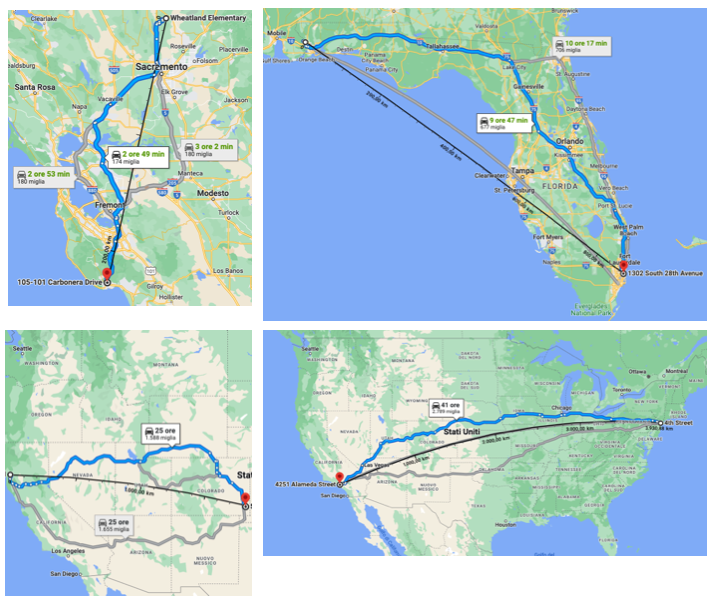
\includegraphics[width=0.65\linewidth]{others/google_maps.png}
			\caption{From left to right top to bottom BAY, FLA, W, USA}
			\label{testpaths}
		\end{figure}
	\end{frame}
	%% %%%%%%%%%%%%%%%%%%%%%%%% %%
	%% CHAPTER 4: SEQUENTIAL A* %%
	%% %%%%%%%%%%%%%%%%%%%%%%%% %%
	\section{A* sequential algorithm}
	\subsection{Data structures}
	\begin{frame}{\secname}
		\framesubtitle{\subsecname}
		%\framesubtitle{Pseudocode}
		The first step consists of a pre-computation of:
		\begin{itemize}
		\item The heuristic $h(n)$ for each node computed through the Haversine formula.
		\item The initial values of $f(n)$ and $g(n)$ that will be set to $DOUBLE\_MAX$ for each
				node except for the source node that will have $f(source) = h(source)$ and $g(source) = 0$.
		\end{itemize}
		Relevant data structures are:
		\begin{itemize}
			\item \textit{costToCome} \texttt{costToCome[i]} contains the current
					best cost to reach node \texttt{i}
			\item \textit{parentVertex}: \texttt{parentVertex[i]} contains the
					parent node of node \texttt{i} according to the current best path found to reach
					the destination
			\item \textit{openSet}: nodes that have to explored (implemented as a Prioriy Queue with
				   $f(n)$ as prioriry)
			\item \textit{closedSet}: already explored nodes 
		\end{itemize}
	\end{frame}
	\subsection{Pseudocode}
	\begin{frame}[allowframebreaks]{\secname}
		\framesubtitle{\subsecname}
		\begin{algorithmic}[1]
			\Function{$astar$}{$G, source, dest, h$}
			\State $g[i] \gets DOUBLE\_MAX \;\forall i \in V$\;
			\State $f[i] \gets DOUBLE\_MAX \;\forall i \in V$\;
			\State $h[i] \gets h(i, d) \; \forall i \in V$\;
			\State $parentVertex[i] \gets -1 \; \forall i \in V$\;
			\State $f[source] \gets h[source]$\;
			\State $g[source] \gets 0$\;
			\State $openSet := \{(source, f[source])\}$\;
			\While{$!openSet.EMPTY()$}
				\State $a \gets openSet.POP()$\;
			\If{$a == dest$}
				\State reconstructPath()\;
				\State return\;
			\EndIf
			\If{$a \in closedSed$}
				\State continue\;
			\EndIf
			\State $closedSed.PUSH(a)$
			\ForAll{neighbors $b$ of $a$}
				\If{$b \in closedSed$}
					\State continue\;
				\EndIf
				\State $wt \gets weight(a, b)$\;
				\State $tentativeScore \gets g[a] + wt$\;
				\If{$tentativeScore < g[b]$}
					\State $parentVertex[b] \gets a$\;
					\State $costToCome[b] \gets wt$\;
					\State $g[b] \gets tentativeScore$\;
					\State $f[b] \gets g[b] + h[b]$\;
					\State $openSet.PUSH((b, f[b]))$\;
				\EndIf
			\EndFor
			\EndWhile
			\EndFunction
		  \end{algorithmic}
	\end{frame}

	\begin{frame}
		\frametitle{4. Sequential A* Algorithm}
		\framesubtitle{Results}
		\begin{table}[ht!]
			\caption{Sequential reading + Sequential A* performance}
			\label{seqtimes}
			\begin{tabular}{|l|l|l|l|l|l|}
			\hline
			\textbf{}    & \textbf{File Size} & \textbf{Reading} & \textbf{A*} & \textbf{Total} & \textbf{\begin{tabular}[c]{@{}l@{}}Reading \\ Impact\end{tabular}} \\ \hline
			\textbf{RND} & 2876B                & 0.0011s           & 0.0519s      & 0.0530s          & 2.1\%                                                           \\ \hline
			\textbf{BAY} & 20.51MB              & 0.9538s           & 0.2197s      & 1.1735s          & 81.3\%                                                         \\ \hline
			\textbf{FLA} & 69.09MB              & 3.1551s           & 0.7174s      & 3.8725s          & 81.5\%                                                           \\ \hline
			\textbf{W}   & 394.26MB             & 18.3065s          & 2.5890s      & 20.8955s         & 87.6\%                                                           \\ \hline
			\textbf{USA} & 1292.40MB            & 56.9942s          & 13.6716s     & 70.6658s         & 80.6\%                                                           \\ \hline
			\end{tabular}
		  \end{table}
		The reading phase has an high impact on the total execution time
	\end{frame}
	%% %%%%%%%%%%%%%%%%%%%%%%%%% %%
	%% CHAPTER 5: A* vs DIJKSTRA %%
	%% %%%%%%%%%%%%%%%%%%%%%%%%% %%
	\section{A* and Dijkstra}
	\subsection{Expanded nodes}
	\begin{frame}{\secname}
		\framesubtitle{\subsecname}
		\begin{table}[ht!]
			\caption{Expanded nodes in different maps}
			\begin{tabular}{|l|l|l|}
			\hline
			\textbf{} & \textbf{Dijkstra} & \textbf{Sequential A*}       \\ \hline
			\textbf{RND}            & 15 of 101           & 13 of 101         \\ \hline
			\textbf{BAY}            & 318725 of 321270    & 157137 of 321270  \\ \hline
			\textbf{FLA}            & 996956 of 1070376   & 592480 of 1070376 \\ \hline
			\textbf{W}              & 5470394 of 1070376  & 1600083 of 1070376 \\ \hline
			\textbf{USA}            & 16676528 of 1070376 & 8998767 of 1070376 \\ \hline
			\end{tabular}
		\end{table}
	\end{frame}
	\begin{frame}{\secname}
		\framesubtitle{\subsecname}
		\begin{figure}[ht!]
			\centering
			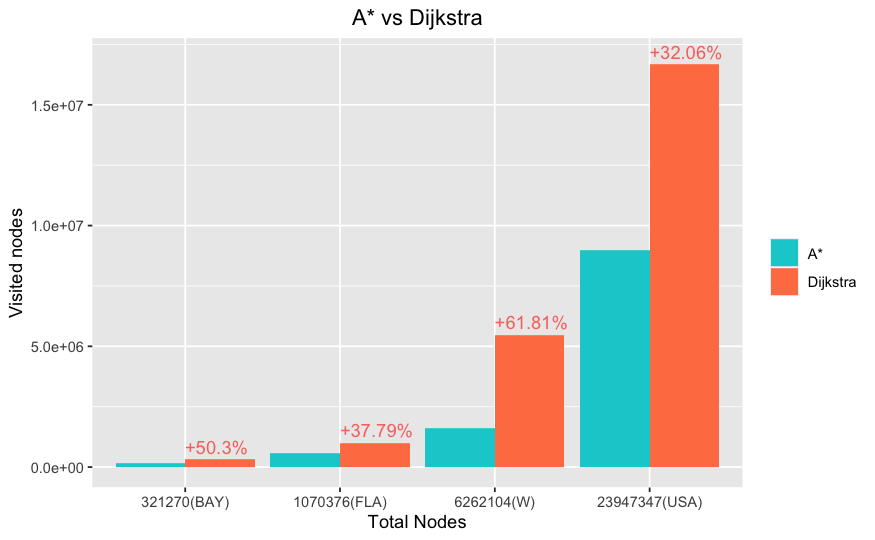
\includegraphics[width=0.8\linewidth]{astar_dijkstra/expanded_nodes.png}
			\caption{Expanded nodes: A* vs Dijkstra}
			\label{histogramnodes}
		\end{figure}
		TODO We can notice that...
	\end{frame}
	\begin{frame}{\secname}
		\framesubtitle{\subsecname}
		\begin{figure}[ht!]
			\centering
			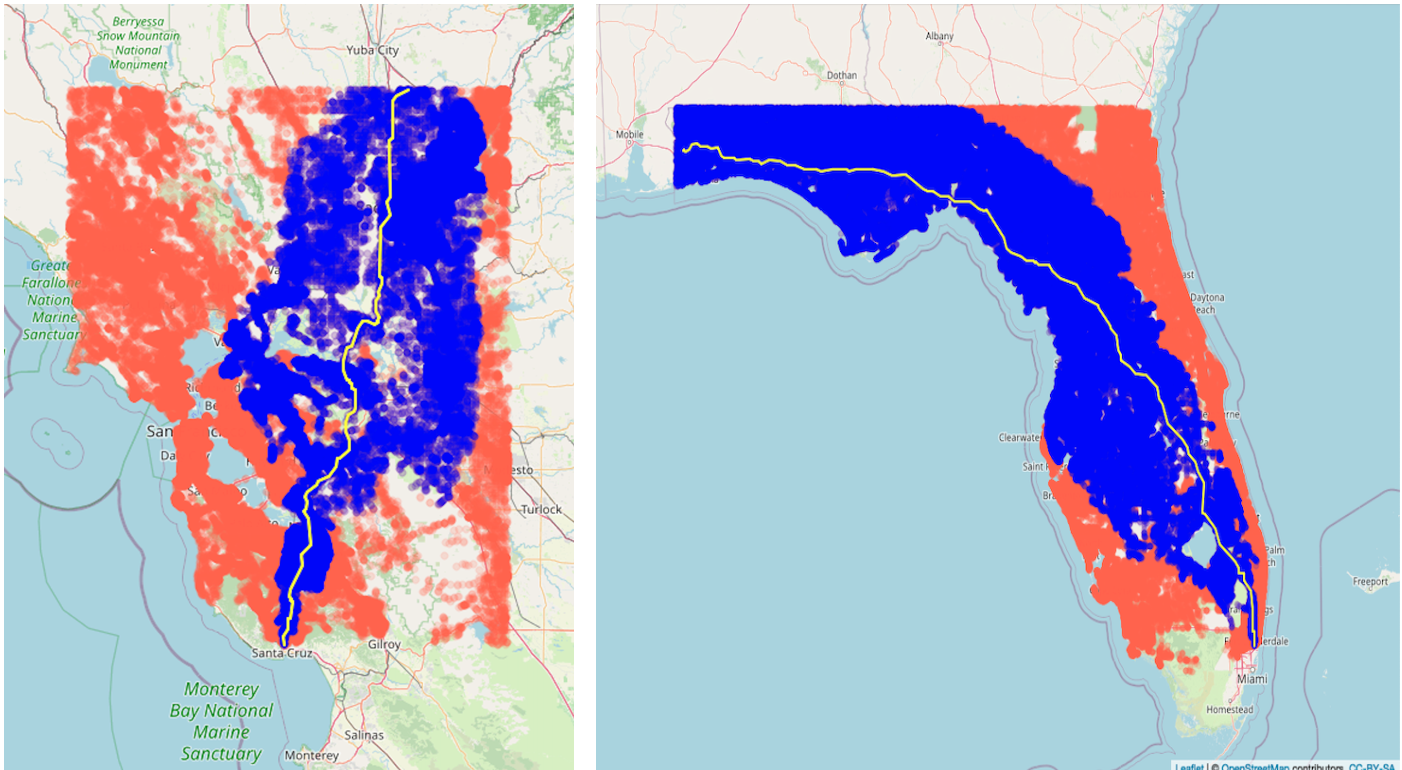
\includegraphics[width=0.8\linewidth]{astar_dijkstra/dijkstra_astar.png}
			\caption{Test paths on BAY(left) and FLA(right)}
			\label{astardijkstra}
		\end{figure}
	\end{frame}
	\subsection{Time and resources comparison}
	\begin{frame}{\secname}
		\framesubtitle{\subsecname}
		\begin{figure}[ht!]
			\centering
			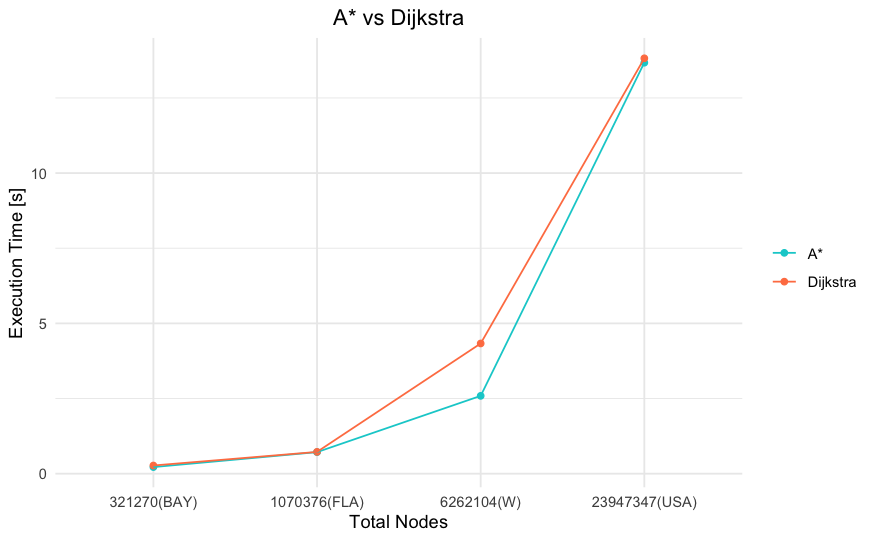
\includegraphics[width=0.8\linewidth]{astar_dijkstra/execution_time.png}
			\caption{Execution time: A* vs Dijkstra}
			\label{astardijkstratime}
		  \end{figure}
	\end{frame}
	\begin{frame}{\secname}
		\framesubtitle{\subsecname}
		\begin{figure}[ht!]
			\centering
			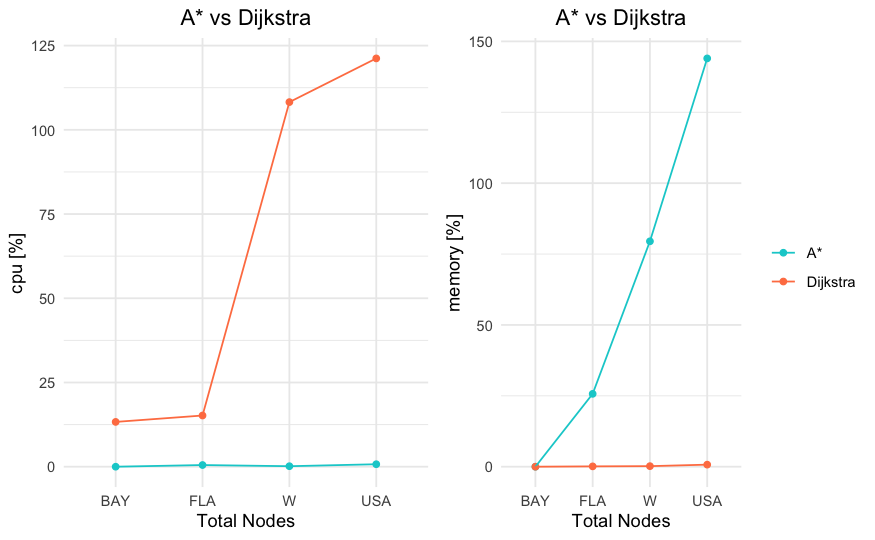
\includegraphics[width=0.8\linewidth]{astar_dijkstra/cpumem.png}
			\caption{Exploited resources: A* vs Dijkstra}
			\label{astardijkstracpumem}
		\end{figure}
	\end{frame}
	%% %%%%%%%%%%%%%%%%%%%%%%%% %%
	%% CHAPTER 6: PARALLEL READ %%
	%% %%%%%%%%%%%%%%%%%%%%%%%% %%
	\section{Parallel input file reading}
	\subsection{Approach 1 (RA1)}
	\begin{frame}{\secname}
		\framesubtitle{\subsecname}
		In this first approach we have implemeted a solution on which:
		\begin{itemize}
			\item The input file is memory-mapped before being read
			\item $N$ threads runs freely to read the entire file (array in RAM)
		\end{itemize}
	\end{frame}
	\subsection{Results on FLA map}
	\begin{frame}{\secname}
		\framesubtitle{\subsecname}
		\begin{figure}[ht!]
			\centering
			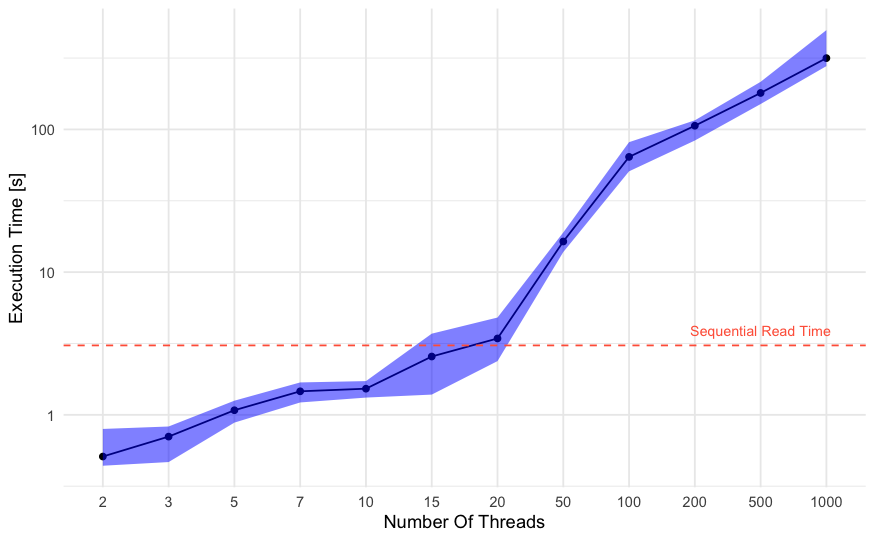
\includegraphics[width=0.85\linewidth]{read/par_read_1_time.png}
			\caption{Performance of RA1 for different number of threads}
			\label{parread1time}
	 	 \end{figure}	
	\end{frame}
	\subsection{Approach 2 (RA2)}
	\begin{frame}{\secname}
		\framesubtitle{\subsecname}
		This is not properly a different approach of parallel reading but simply a version
		of the \textit{RA1} needed when the \textit{PNBA*} algorithm will be applied:
		\begin{itemize}
			\item The input file is memory-mapped before being read
			\item $N$ threads runs freely to read the entire file (array in RAM)
			\item Two different graphs are loaded: $G$ and the reversed graph $R$
		\end{itemize}
		Since we are loading two graphs data structures at the same time the performances will
		compared with the sequential reading as if it was run twice (the first time to read $G$ and
		the second time to read $R$)
	\end{frame}
	\subsection{Results on FLA map}
	\begin{frame}{\secname}
		\framesubtitle{\subsecname}
		\begin{figure}[ht!]
			\centering
			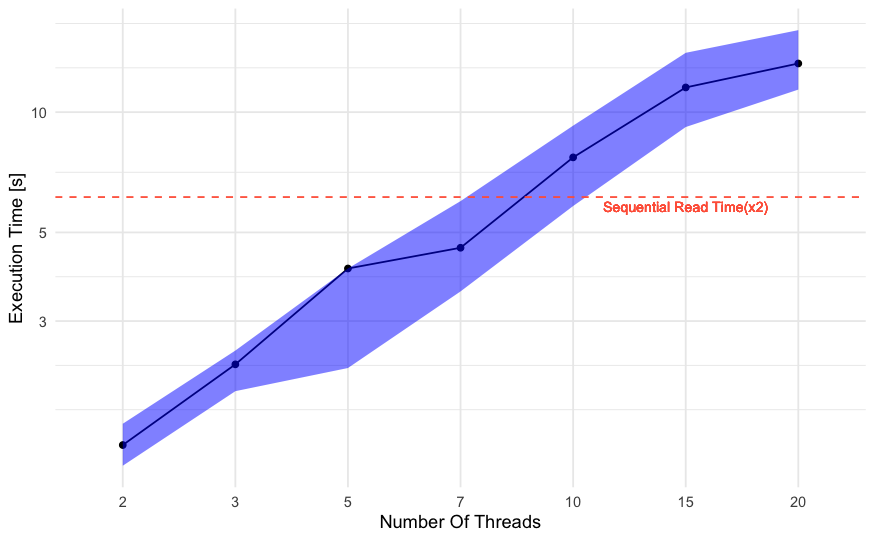
\includegraphics[width=0.8\linewidth]{read/par_read_2_time.png}
			%\caption{Performance of approach 2 for different number of threads}
			\label{parread2time}
		  \end{figure}
	\end{frame}
	\subsection{RA1 and RA2 on FLA map}
	\begin{frame}{\secname}
		\framesubtitle{\subsecname}
		\begin{figure}[ht!]
			\centering
			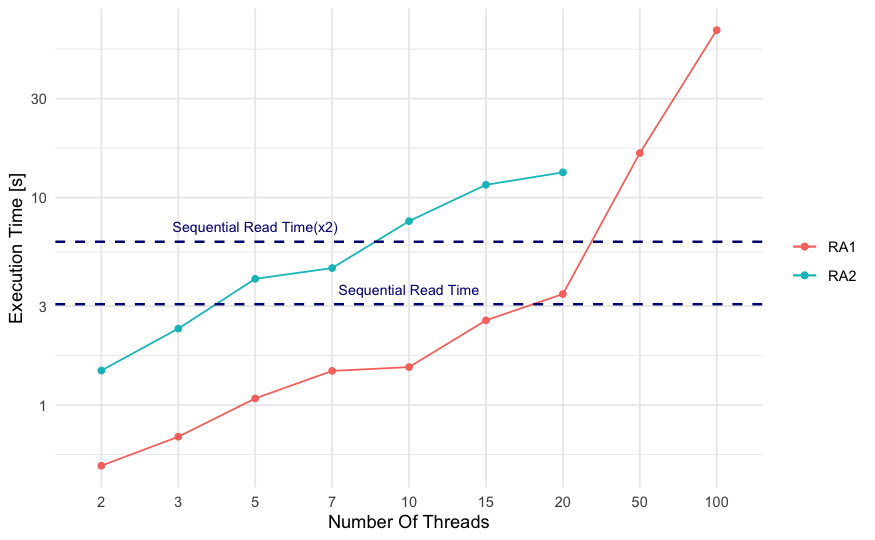
\includegraphics[width=1\linewidth]{read/par_read_all_time.png}
			\caption{RA(Read Approach) 1,2,3 compared with sequential reading}
			\label{parreadalltime}
		\end{figure}
	\end{frame}
	\subsection{Results on all maps}
	\begin{frame}{\secname}
		\framesubtitle{\subsecname}
		\begin{table}[ht!]
			\centering
			  \caption{RA1 results against sequential reading}
			  \begin{tabular}{|l|l|l|l|}
			  \hline
			  \textbf{}    & \textbf{\begin{tabular}[c]{@{}l@{}}RA1\\ (2 threads)\end{tabular}} & \textbf{Sequential} & \textbf{Speed-Up} \\ \hline
			  \textbf{BAY} & 0.1936s                                                            & 0.9366s             & 79.3\%            \\ \hline
			  \textbf{FLA} & 0.5103s                                                            & 3.0650s             & 83.4\%            \\ \hline
			  \textbf{W} & 3.3303s                                                              & 17.8834s            & 81.4\%            \\ \hline
			  \textbf{USA} & 14.1492s                                                           & 56.4445s            & 74.9\%            \\ \hline
			  \end{tabular}
			  \label{readresultsfinal}
		  \end{table}
	\end{frame}
	\begin{frame}{\secname}
		\framesubtitle{\subsecname}
		\begin{table}[ht!]
			\centering
			  \caption{RA2 results against sequential reading}
			  \begin{tabular}{|l|l|l|l|}
			  \hline
			  \textbf{}    & \textbf{\begin{tabular}[c]{@{}l@{}}RA2\\ (2 threads)\end{tabular}} & \textbf{Sequential(x2)} & \textbf{Speed-Up} \\ \hline
			  \textbf{BAY} & 0.5313s                                                           & 1.8732s              & 71.6\%            \\ \hline
			  \textbf{FLA} & 1.4682s                                                            & 6.1300s             & 76.1\%            \\ \hline
			  \textbf{W} & 10.4959s                                                             & 35.7668s            & 70.7\%            \\ \hline
			  \textbf{USA} & 35.4505s                                                           & 112.8890s            & 68.6\%            \\ \hline
			  \end{tabular}
			  \label{readresultsfinal}
		  \end{table}
	\end{frame}
	\begin{frame}{\secname}
		\framesubtitle{\subsecname}
		\begin{figure}[ht!]
			\centering
			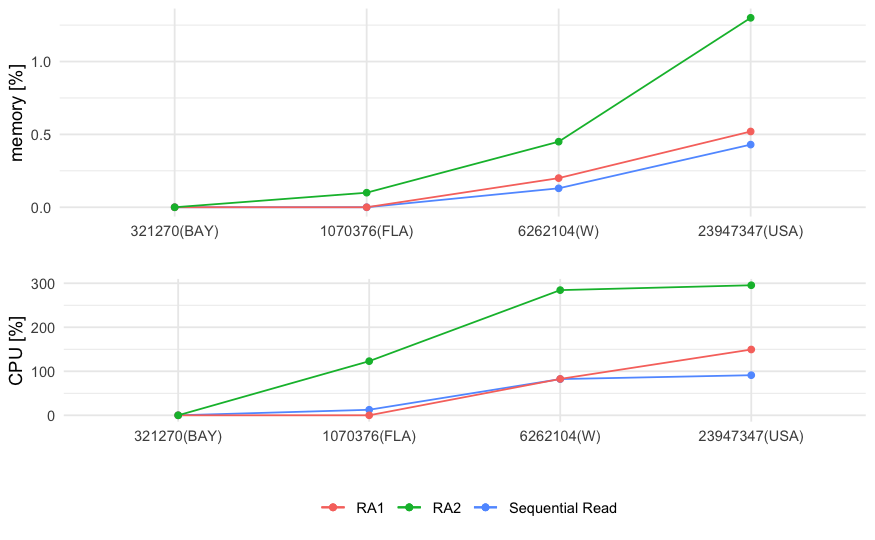
\includegraphics[width=1\linewidth]{read/parread_cpumem.png}
			\caption{RA(Read Approach) 1,2 compared with sequential reading on FLA - exploited resources}
			\label{parreadallcpumem}
		  \end{figure}
	\end{frame}
	%% %%%%%%%%%%%%%%%%%%%%%% %%
	%% CHAPTER 7: PARALLEL A* %%
	%% %%%%%%%%%%%%%%%%%%%%%% %%
	\section{Parallel A*}
	\begin{frame}{\secname}
		The goal of the project was to find one or more parallel versions of the A* algorithm 
		and showing their performances w.r.t. the sequential version. We have followed two approaches
		to face this problem:: 
		\begin{itemize}
			\item \textbf{Hash Distributed A* (HDA*)}: it puts in action a complex way of parallelizing A* by defining a hash-based work distribution strategy.
		    \item \textbf{Parallel New Bidirectional A* (PNBA*)}: parallel search of the path from \textit{source} to \textit{dest}
				  and of the path from \textit{dest} to \textit{source} in the reversed graph.
		\end{itemize}
	\end{frame}
	\subsection{HDA*}
	\begin{frame}{\secname : \subsecname}
		%\framesubtitle{\subsecname}
		\begin{itemize}
			\item \textit{Ownership}: HDA* work is based on the fact that each thread is \textit{owner} of a
				  specific set of nodes of the Graph -> given a node $n$ it is defined a hash function $f:\;f(n) = t$
				  where $t \in \{1..N\}$ with $N$ the number of threads
			\item When a thread extracts from the \textit{open set}
			      (expands) a node all its neighbors are added to the \textit{open set} of the owner thread of the expanded node.
		\end{itemize}
	\end{frame}
	\begin{frame}{\secname : \subsecname}
		%\framesubtitle{\subsecname} 
		HDA* doesn't provide the same guarantees of the sequential algorithm:
		\begin{itemize}
		\item   In sequential A* if it's provided an heuristic function that is both \textit{admissible}
				and \textit{consistent} we have the guarantee that each node will be only expanded once
				and that the first time we expand that node we have found a shortest path to it.
		\item   In HDA* we loose these guarantees: since we don't know in which order nodes will be processed
				it could happen that a longer path to \textit{dest} is found before the shortest one so
				a node could be opened more than once and expanding the \textit{dest} node doesn't
				mean that we have terminated.
		\end{itemize}
	\end{frame}
	\subsubsection{The hash function}
	\begin{frame}{\secname : \subsecname}
		\framesubtitle{The hash function} 
		We have implemented two types of hash functions:
		\begin{block}{Hash functions definitions}
			$hash_1(node\_index, num\_threads) = node\_index \;\%\; num\_threads$
			$hash_2(node\_index, num\_threads, V) = i-1 \;with\;
			i = min_i : \frac{V}{num\_threads}\cdot i > node\_index \;, i \in \{1,...,num\_threads\}$
		\end{block}
		\begin{itemize}
			\item The first one simply assigns a node to a thread in a randomic fashion w.r.t to its position
				  inside the map
			\item What tries to do the second hash function (the one that we have used to 
				  measure performances) is simply assigning nodes to threads following their index
				  numbering (e.g. nodes from $0$ to $K$ to thread $t_0$, nodes from
				  $K+1$ to $H$ to thread $t_1$ and so on and so forth).
		\end{itemize}
	\end{frame}
	\subsubsection{Work distribution on BAY map}
	\begin{frame}{\secname : \subsecname}
		\framesubtitle{Work distribution on BAY map}
		\begin{figure}[ht!]
			\centering
			\small
			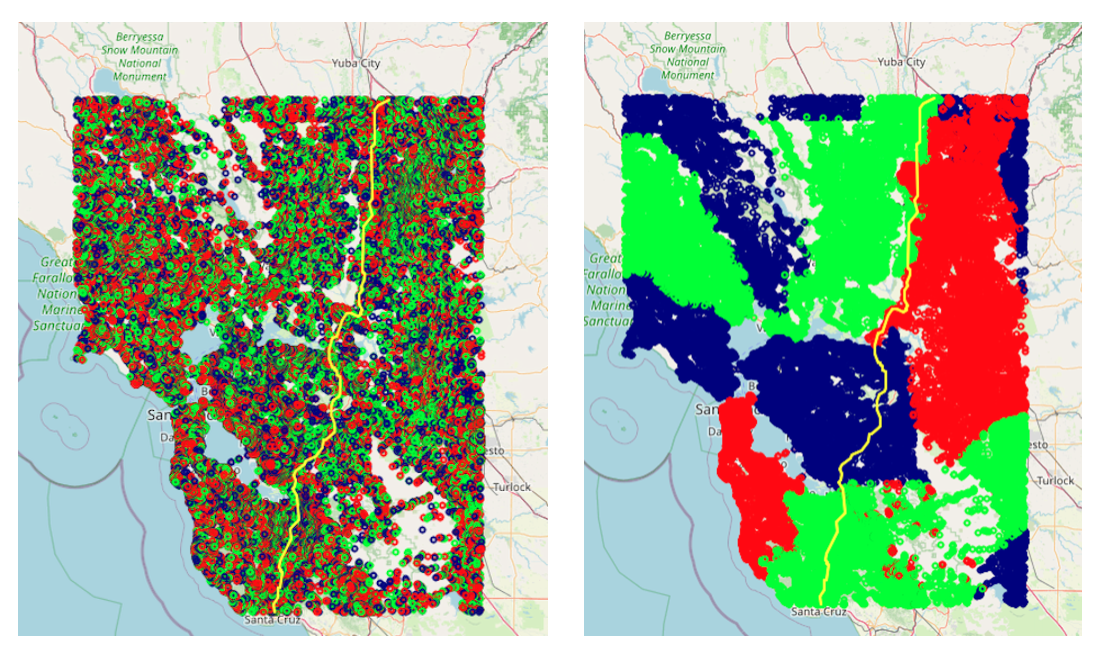
\includegraphics[width=0.8\linewidth]{hda/hda_work_BAY.png}
			\caption{HDA* work distribution among 3 threads in BAY map}
			\label{hdawork1}
		  \end{figure}
	\end{frame}
	\subsubsection{Distributed termination condition}
	\begin{frame}{\secname : \subsecname}
		\framesubtitle{Distributed termination condition}
		\begin{itemize}
			\item \textbf{Barrier method (B)}: when a thread realizes that its \textit{open set} is
			empty a barrier is 
			hitten and when all the threads have hitten the barrier
			each one makes a check to confirm(or not) that all the \textit{open sets} of all
			the threads are still empty. If this is not true it means that there are nodes
			that have still to be processed and the best path to $dest$ found so far could
			not be the optimal one otherwise all the threads can terminate.
			\item \textbf{Sum-Flag method (SF)}: the idea behind the sum flag method comes from the fact that
			the Barrier mechanism could be quite expensive. In this termination condition method
			each thread keeps a binary flag saying whether its \textit{open set} is empty
			or not. When no more nodes are inside it the flag is set and if $\sum_{i=1}^{N}flag[i] = N$
			all the threads can correctly terminate.
		\end{itemize}
	\end{frame}
	\subsubsection{Duplicate nodes}
	\begin{frame}{\secname : \subsecname}
		\framesubtitle{Duplicate nodes}
		We also need to check whether the cost associated to an expanded node 
		when it was previously added to the \textit{closed set} is less or equal to the cost computed at the time $n$ is re-expanded. 
		This is called duplicate checking so, a node $n$ is a duplicate of node $m$ if:
		\begin{itemize} 
			\item $n$ is equal to $m$
			\item $closedSet$ of thread $t_i$ contains the node $m$
			\item $g(m) \le g(n)$
		\end{itemize}
		A duplicate node can be discarded.
	\end{frame}
	\subsubsection{Communication methodology}
	\begin{frame}{\secname : \subsecname}
		\framesubtitle{Communication methodology}
		\begin{itemize}
			\item \textbf{Shared Address Space (SAS)}: threads share pointers to common data structures (we need
			to cope with mutual exclusion)
			\item \textbf{Message Passing (MP)}: threads can communicate only through messages and don't share any
				   data structure
		\end{itemize}
	\end{frame}
	\subsubsection{Shared Address Space (SAS)}
	\begin{frame}{\secname : \subsecname}
		\framesubtitle{Shared Address Space (SAS)}
		The shared data structures are:
		\begin{itemize}
			\item A global array of \textit{open sets} that here we call $A$ where
				  $A[i]$ contains a pointer to the \textit{open set} of thread $t_i$ and the size
				  of $A$ is $N$ (the number of threads).
			\item The $parentVertex$ and $costToCome$ data structures are shared among all the threads.
		\end{itemize}
		This approach clearly requires locks so that the operations on the shared data structures
		can happen in mutual exclusion. In particular we need:
		\begin{itemize}
			\item One lock $L1$ for each \textit{open set} so for each $A[i] \;\forall i \in \{1..N\}$.
			\item One lock $L2$ for each node of the graph in order to correctly update $parentVertex$ and $costToCome$ data structures.
		\end{itemize}
	\end{frame}
	\subsubsection{SAS pseudocode}
	\begin{frame}[allowframebreaks]{\secname : \subsecname}
		\framesubtitle{SAS pseudocode}
		\begin{algorithmic}[1]
			\Function{$astar$}{$G, source, dest, h$}
				\State $g[i] \gets DOUBLE\_MAX \;\forall i \in V$\;
				\State $h[i] \gets heuristic(i, dest) \; \forall i \in V$\;
				\State $parentVertex[i] \gets -1 \; \forall i \in V$\;
				\State $t\_owner \gets hash(source, num\_threads)$\;
				\State $f[t\_owner][source] \gets h[s]$\;
				\State $g[source] \gets 0$\;
				\State $openSet[t\_owner] := \{(source, f[t\_owner][source])\}$\;
				\State Initialize $N$ $mutex\_threads$\;
				\State Initialize $V$ $mutex\_nodes$\;
				\State Launch $N$ threads\;
				\State Join $N$ threads\;
				\State $reconstructPath()$\;
			\EndFunction
			\Function{$hda\_sas$}{}
				\While{$1$}
      				\While{$!openSet[index].EMPTY()$}
        				\State LOCK($mutex\_threads[index]$)\;
        				\State $a \gets openSet.POP()$\;
        				\State UNLOCK($mutex\_threads[index]$)\;
      				\EndWhile
      			\If{$a$ is duplicate}
        			\State continue\;
      			\EndIf
      		    \For{neighbor $b$ of $a$}
        			\State $wt \gets weight(a, b)$\;
        			\State $tentativeScore \gets g[a] + wt$\;
        			\If{$tentativeScore$ is less than $g[b]$}
          				\State $owner\_a \gets hash(a,N)$\;
          				\State $owner\_b \gets hash(b,N)$\;
					\EndIf
          			\If{$b$ is duplicate}
            			\State continue\;
          			\EndIf
          			\State LOCK($mutex\_nodes[a]$)\;
          			\State $tentativeScore \gets g[a] + wt$\;
          			\State UNLOCK($mutex\_nodes[a]$)\;

          			\State LOCK($mutex\_nodes[b]$)\;
          			\If{$tentativeScore$ is less than $g[b]$}
					    \State $parentVertex[b] \gets a$\;
            			\State $costToCome[b] \gets wt$\;
            			\State $g[b] \gets tentativeScore$\;
            			\State $f[b] \gets g[b] + h[b]$\;
            			\State LOCK($mutex\_threads[owner\_b]$)\;
            			\State $f[owner\_b][b] \gets f[b]$\;
            			\State $openSet.PUSH((b, f[owner\_b][b]))$\;
            			\State UNLOCK($mutex\_threads[owner\_b]$)\;
          			\EndIf
          			\State UNLOCK($mutex\_nodes[b]$)\;
        		\EndFor
				\EndWhile

      		\If{$openSet[index].EMPTY()$ and $parentVertex[dest] != -1$}
        		\State Terminate according to B or SF\;
      		\EndIf
		  \EndFunction
		  \end{algorithmic}
	\end{frame}
	\subsubsection{Results}
	\begin{frame}{\secname : \subsecname}
		\framesubtitle{Results}
		\begin{figure}[ht!]
			\centering
			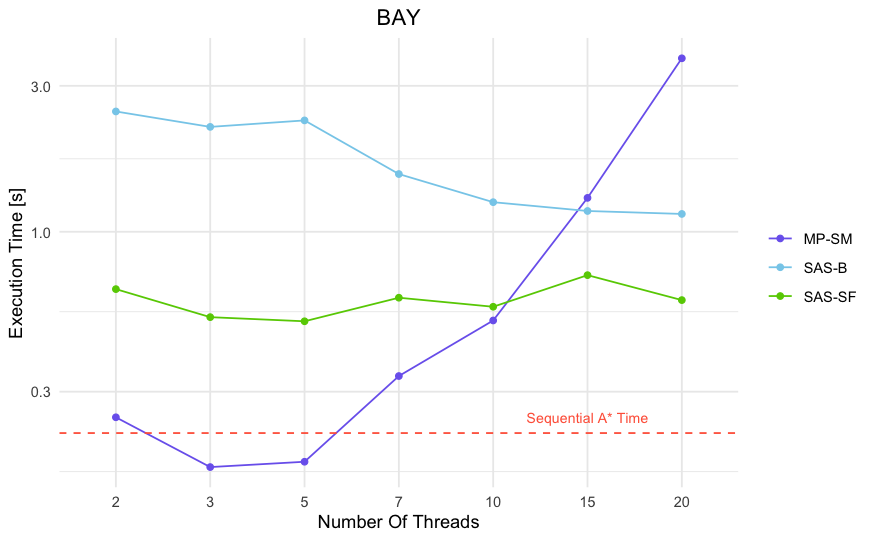
\includegraphics[width=0.8\linewidth]{hda/baytime.png}
			\caption{HDA* on BAY map}
		\end{figure}
	\end{frame}
	\begin{frame}{\secname : \subsecname}
		\framesubtitle{Results}
		\begin{figure}[ht!]
			\centering
			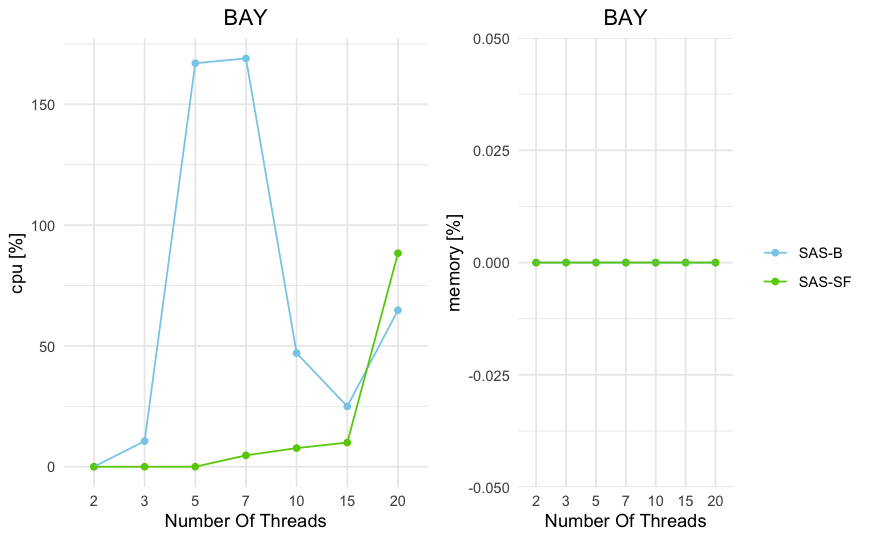
\includegraphics[width=0.8\linewidth]{hda/baycpumem.png}
			\caption{HDA* on BAY map}
		\end{figure}
	\end{frame}
	\begin{frame}{\secname : \subsecname}
		\framesubtitle{Results}
		\begin{figure}[ht!]
			\centering
			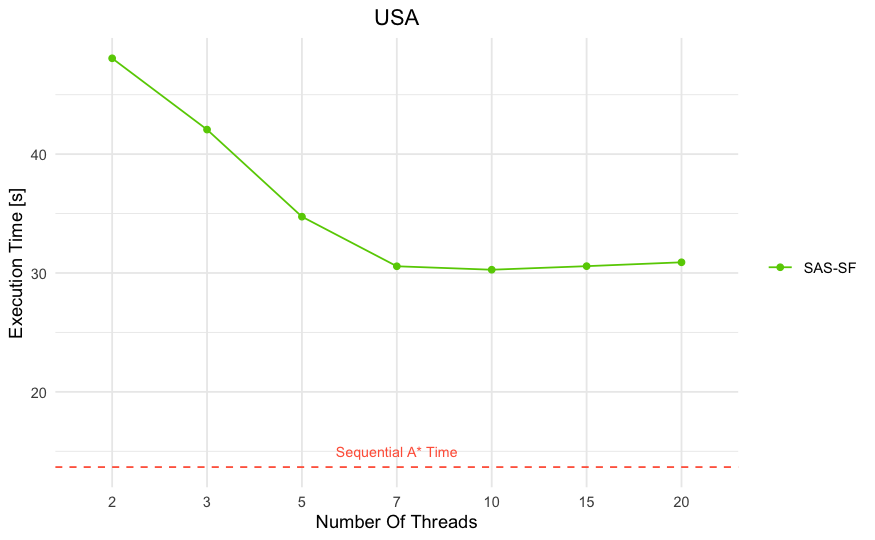
\includegraphics[width=0.8\linewidth]{hda/usatime.png}
			\caption{HDA* on USA map}
		\end{figure}
	\end{frame}
	\begin{frame}{\secname : \subsecname}
		\framesubtitle{Results}
		\begin{figure}[ht!]
			\centering
			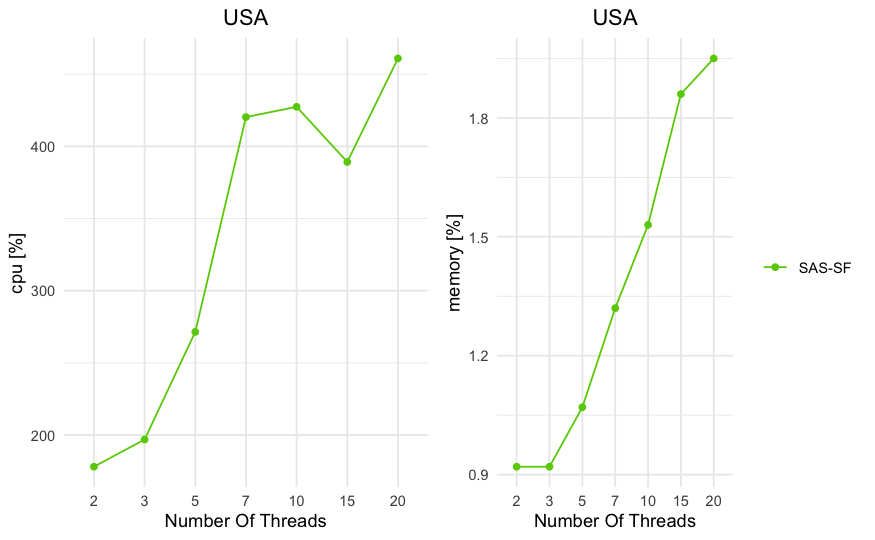
\includegraphics[width=0.8\linewidth]{hda/usacpumem.png}
			\caption{HDA* on USA map}
		\end{figure}
	\end{frame}
	\subsubsection{Comments and overall results}
	\begin{frame}{\secname : \subsecname}
		\framesubtitle{Comments and overall results}
		\begin{itemize}
		\item The SAS-MP variant of HDA* is not scalable.
		\item The SAS-B is more scalable
				than SAS-MP but the termination condition is not well-performing on large graphs.
		\item The SAS-SF behaves overall better.
				Despite the fact that on maps BAY, FLA, W it is difficult to notice the improvements when
				the number of threads increases this is more evident on USA map. Performances are always
				better compared to the SAS-B algorithm.
		\item About the resource consumption both SAS-B and SAS-SF are more expensive in terms on CPU and 
				memory used w.r.t the sequential algorithm. The resource used increase as the number of threads
				increase.
		\end{itemize}
	\end{frame}
	\begin{frame}{\secname : \subsecname}
		\framesubtitle{Comments and overall results}
		Here we only write the performances of SAS-SF that is the only one able to achieve reasonable results
		on all the benchmark graphs:
		\begin{table}[ht!]
			\centering
			\caption{SAS-SF with best number of threads time performances}
			\begin{tabular}{|l|l|l|l|l|}
			\hline
			\textbf{}    & \textbf{Threads} & \textbf{SAS-SF} & \textbf{Sequential A*} & \textbf{Slow-Down}\\ \hline
			\textbf{BAY} & 5        & 0.5097s                & 0.2647s  &92.6\%          \\ \hline
			\textbf{FLA} & 7        & 1.6383s                & 0.7174s  & 128.3\%          \\ \hline
			\textbf{W}   & 7        & 10.8626s                & 2.5890s &319.6\%           \\ \hline
			\textbf{USA} & 7         & 30.5655s               & 13.6716 &123.6\%           \\ \hline
			\end{tabular}
			\label{tablesas}
		  \end{table}
	\end{frame}
	\begin{frame}{\secname : \subsecname}
		\framesubtitle{Comments and overall results}
		\begin{figure}[ht!]
			\centering
			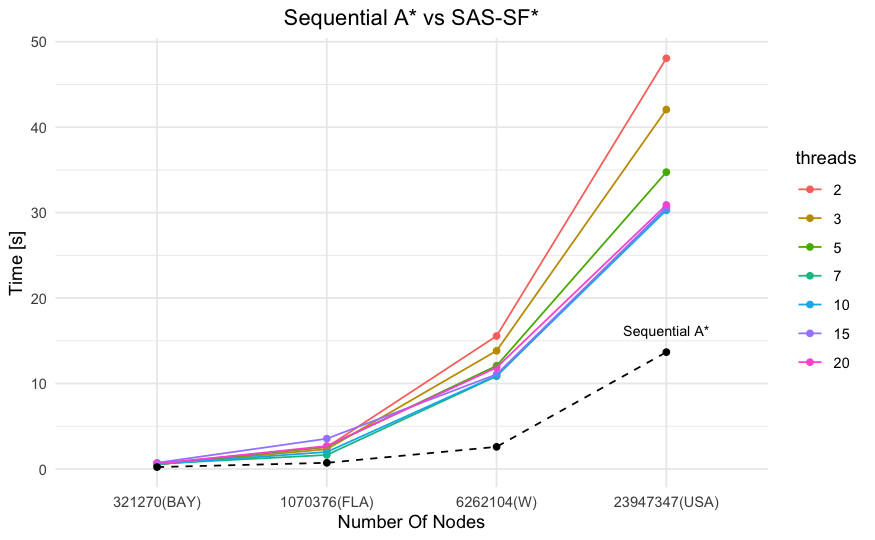
\includegraphics[width=0.8\linewidth]{hda/tottime.png}
			\caption{HDA* overall performances}
		\end{figure}
	\end{frame}
	\begin{frame}{\secname : \subsecname}
		\framesubtitle{Comments and overall results}
		\begin{figure}[ht!]
			\centering
			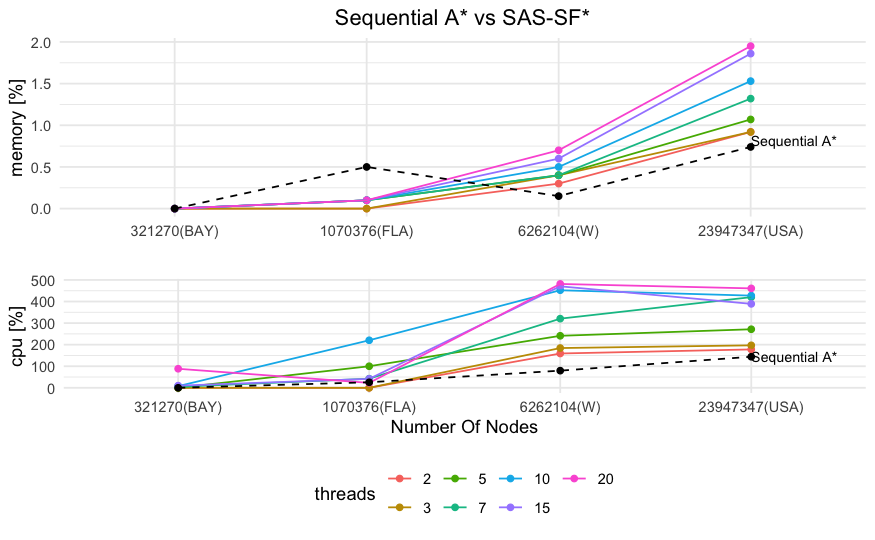
\includegraphics[width=0.8\linewidth]{hda/totcpumem.png}
			\caption{HDA* ooverall performances}
		\end{figure}
	\end{frame}
	\begin{frame}{\secname : \subsecname}
		\framesubtitle{Comments and overall results}
		\begin{itemize}
			\item The hash function has an important impact on the performances of A* algorithm. The one that
				  we have used is probably not optimal. Using a more efficient one could lead to obtain better performances but we
				  suppose that the sequential algorithm would still be the "best case" instead of being the "worst case"
				  in terms of execution time. 
			\item The termination condition is clearly a bottleneck, in particular if the Barrier method
				  is used. This can be less evident with small maps but we can appreciate it on bigger graphs.
			\item By increasing the number of threads both SAS-SF and SAS-B perform better in terms of execution time (even if
				  the resource consumption increases) but this is not enough: the performance scalability
				  and improvements that should have been obtained with large graphs have not been verified.
		  \end{itemize}
	\end{frame}
	%% %%%%%%%%%%%%%%%%%%%%%% %%
	%% CHAPTER 7: PARALLEL A* %%
	%% %%%%%%%%%%%%%%%%%%%%%% %%
	\subsection{PNBA*}
	\subsubsection{NBA*}
	\begin{frame}{\secname : \subsecname}
		\framesubtitle{NBA*}
		The NBA* algorithm is a version of  the bidirectional search that uses a data
		structure $M$ to keep track of the nodes in the middle between the two searcher
		threads $t_G$ and $t_R$. $M$ initially contains all the nodes of the graph. The nodes
		in the search frontiers are the ones that:
		\begin{itemize}
		\item Belongs to $M$
		\item Have been labelled: $g_G(n) < \infty $ or $g_R(n) < \infty $
		\end{itemize}
		The threads $t_G$ and $t_R$ share a variable $L$ initialized to $\infty$ that contains
		the cost of the best path from $source$ to $dest$. Other common variables are:
		\begin{itemize}
		\item $F_G$: lowest $f_G$ value on $t_G$ frontier.
		\item $F_R$: lowest $f_R$ value on $t_R$ frontier.
		\item Variables $F_p$, $f_p$, $g_p$ (with $p \in \{R,G\}$) are written on only one
				side but read by both sides.
		\end{itemize}
	\end{frame}
	\begin{frame}{\secname : \subsecname}
		\framesubtitle{NBA*}
		These are the initialization steps done by $t_G$ (same for $t_R$)
		\begin{itemize}
		\item $g_G(source_G)=0$, $F_G(source_G)=f_G(source_G)$
		\end{itemize}
		At each iteration it is extracted a node $x$ such that:
		\begin{itemize}
		\item $x \in M$
		\item $x: f_G(x) = min f_G(v) \forall v \in openSet_G$ 
		\end{itemize}
		The node is removed from $M$ and pruned (not expanded) if $f_G(x) \ge L$ or
		$g_G(x)+F_R-h_R(x) \ge L$. Otherwise all its successors $y$ are generated. In the
		first case it is classified as \textit{rejected} while in the other situation it is
		\textit{stabilized} because $g_G(x)$ won't be changed anymore. For each $y$ we update:
		\begin{itemize}
		\item $g_G(x)$: $min(g_G(y), g_G(x) + d_G(x, y))$
		\item $L$: $min(L, g_G(x) + g_G(y))$
		\end{itemize}
		The algorithm stops when no more candidates have to be expanded in one of the two sides.
	\end{frame}
	\subsubsection{PNBA*}
	\begin{frame}{\secname : \subsecname}
		\framesubtitle{PNBA*}
		The PNBA* algorithm improves the NBA* algorithm by letting the two threads working in
		parallel (and not in an alternate mode). This requires to cope with mutual exclusion on some data.
		\begin{figure}[ht!]
			\centering
			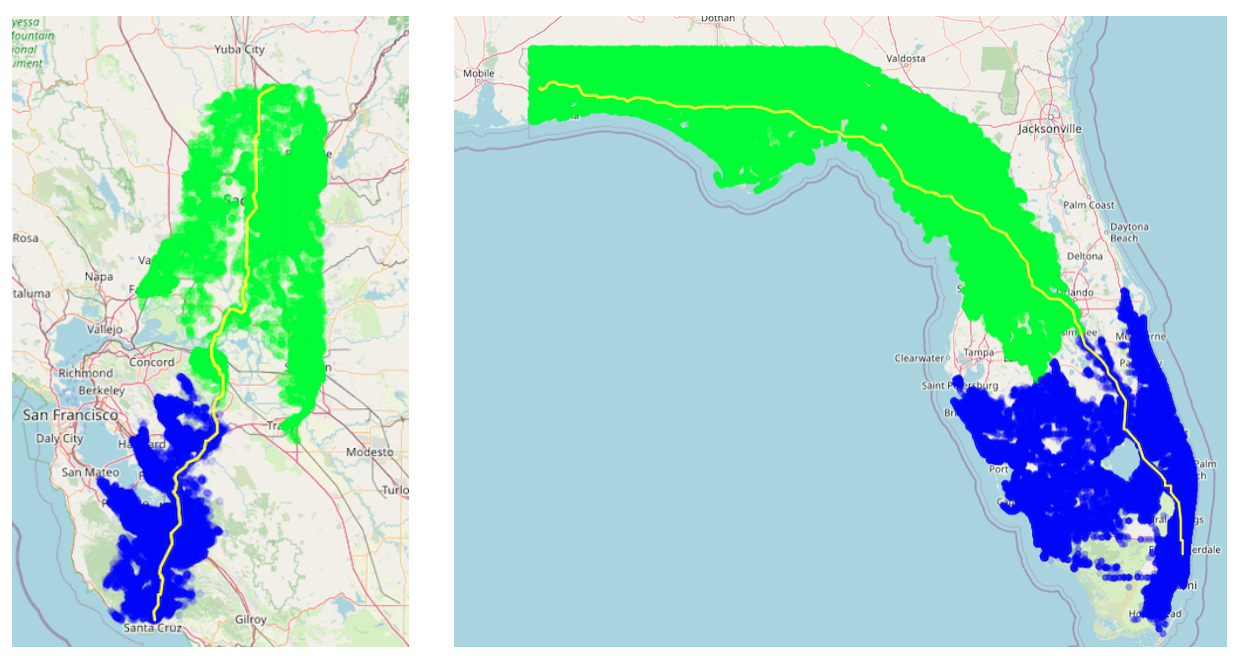
\includegraphics[width=0.7\linewidth]{pnba/pnbamap.png}
			\caption{PNBA* work on BAY(left) and FLA(right)}
			\label{pnbamap}
		\end{figure}
	\end{frame}
	\subsubsection{PNBA* pseudocode}
	\begin{frame}[allowframebreaks]{\secname}
		\framesubtitle{\subsecname}
		\begin{algorithmic}[1]
			\Function{$pnba_G()$}{}
				\While{$!finished$}
					\State $x \gets openSet_G.POP()$\; 
					\If{$x \in M$} 
							\If{$(f_G(x) < L) \wedge (g_G(x) + F_R - h_R(x) < L$)}
								\For{all edges $(x, y)$}
									\If{$(y \in M) \wedge (g_G(x) > g_G(x) + d_G(x, y)$}
										\State $g_G(y) \gets g_G(x) + d_G(x, y)$
										\State $f_G(y) \gets g_G(x) + h_G(x, y)$
										\If{$y \in openSet_G$}
											\State $openSet_G.REMOVE(y)$
										\EndIf
										\State $openSet_G.PUSH(\{f_G(y), y\})$
										\If{$g_G(y) + g_R(y) < L$}
											\State $lock$\;
											\If{$g_G(y) + g_R(y) < L$}
												\State $L \gets g_G(y) + g_R(y)$\;
											\EndIf
											\State $unlock$\;
										\EndIf
									\EndIf
								\EndFor
							\EndIf
							\State $ M \gets M - \{x\}$\;
					\EndIf
					\If{$!openSet_G.EMPTY()$}
						\State $F_G \gets f[openSet_G.PEEK()]$\;
						\Else
						 	\State $finished \gets true$\;
					\EndIf
				\EndWhile
			\EndFunction
		  \end{algorithmic}
	\end{frame}
	\begin{frame}{\secname : \subsecname}
		\framesubtitle{Results}
		\begin{itemize}
			\item The PNBA* is able to outperform the sequential algorithm in terms of execution time in all the 
				  graphs we have tested it on.
			\item The speed-up increases as the number of nodes increases and this can 
				  be a good news if we will try to implement it on much bigger graps.
			\item The execution time and the number of
				  nodes have been proved to strongly depend on the position of the common node found. Best performances
				  are achieved when the common node found is approximately in between of source and destination nodes.
			\item Resource consumption is almost 2x w.r.t. the sequential algorithm and this is reasonable considering
				  that it is like running two sequential algorithm in concurrency
		\end{itemize}
	\end{frame}
	\begin{frame}{\secname : \subsecname}
		\framesubtitle{Results}
		\begin{table}[ht!]
			\centering
			\caption{PNBA* - time performances}
			\begin{tabular}{|l|l|l|l|}
			\hline
			\textbf{}    & \textbf{PNBA*} & \textbf{Sequential A*} & \textbf{Speed-Up} \\ \hline
			\textbf{BAY} & 0.2091s        & 0.2197s                & 4.82\%            \\ \hline
			\textbf{FLA} & 0.6782s        & 0.7174s                & 5.46\%            \\ \hline
			\textbf{W}   & 2.3029s        & 2.5890s                & 11.1\%            \\ \hline
			\textbf{USA} & 9.0568         & 13.6716s               & 33.8\%            \\ \hline
			\end{tabular}
		  \end{table}
	\end{frame}
	\begin{frame}{\secname : \subsecname}
		\framesubtitle{Results}
		\begin{figure}[ht!]
			\centering
			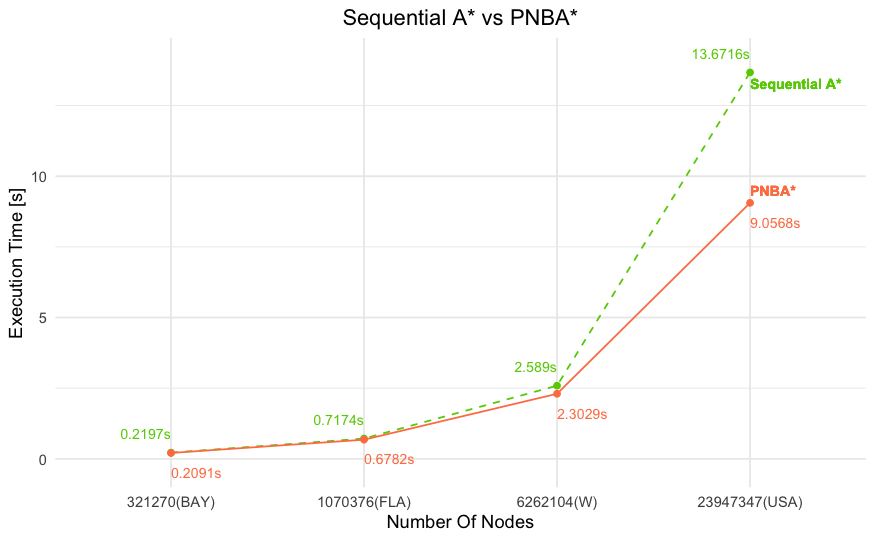
\includegraphics[width=0.85\linewidth]{pnba/pnba_time.png}
			\caption{PNBA* overall performances}
		  \end{figure}
	\end{frame}
	\begin{frame}{\secname : \subsecname}
		\framesubtitle{Results}
		\begin{figure}[ht!]
			\centering
			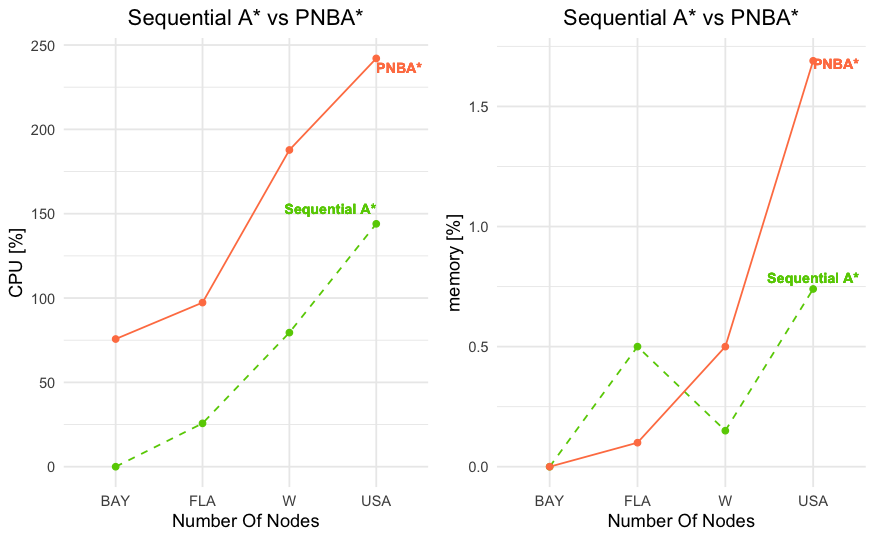
\includegraphics[width=0.85\linewidth]{pnba/pnba_cpumem.png}
			\caption{PNBA* overall performances - time}
		  \end{figure}
	\end{frame}
	%% %%%%%%%%%%%%%%%%%%%%%% %%
	%% CHAPTER 8: CONCLUSIONS %%
	%% %%%%%%%%%%%%%%%%%%%%%% %%
	\section{Conclusions}
	\begin{frame}{\secname}
		\begin{figure}[ht!]
			\centering
			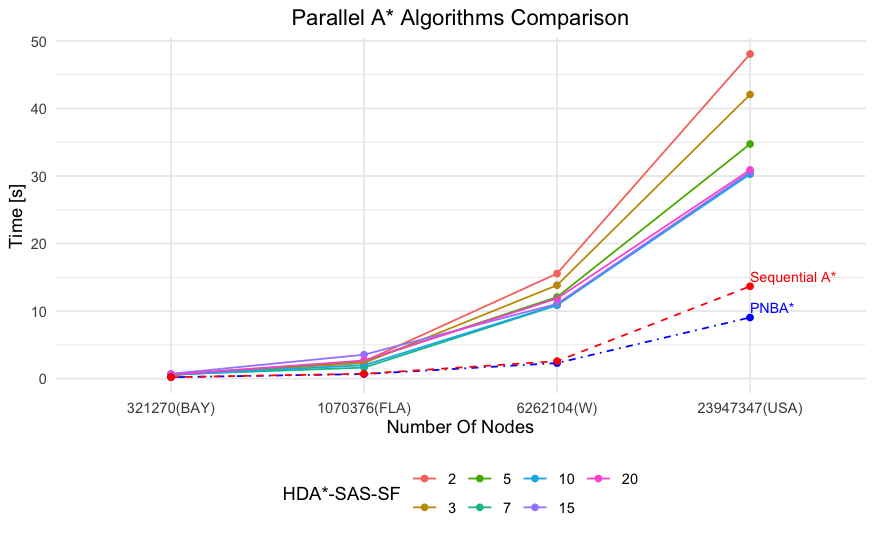
\includegraphics[width=0.85\linewidth]{others/allalgo_time.png}
			\caption{Parallel A* overall performances - resources}
		\end{figure}
	\end{frame}
	\begin{frame}{\secname}
		\begin{figure}[ht!]
			\centering
			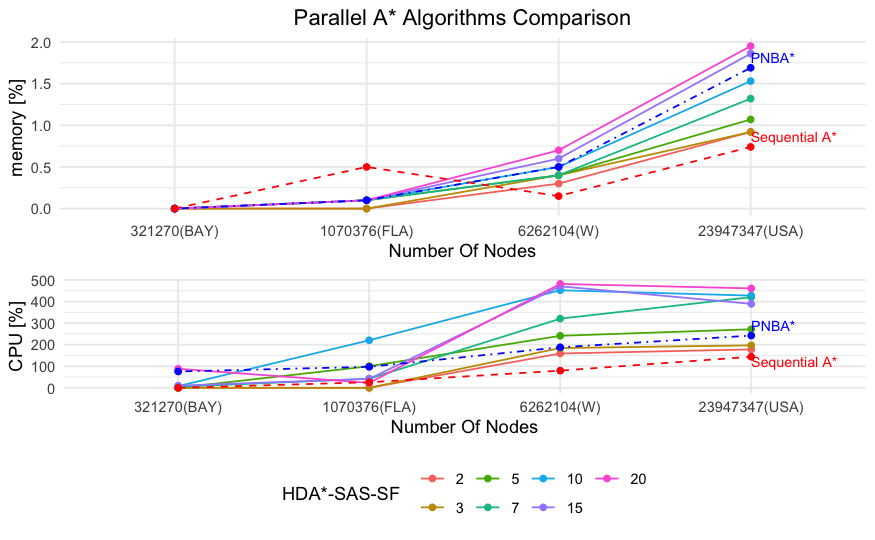
\includegraphics[width=0.85\linewidth]{others/allalgo_cpumem.png}
			\caption{Parallel A* overall performances}
		\end{figure}
	\end{frame}
	%% %%%%%%%%%%%%%%%%%%%%%%%%%%%%%%% %%
	%% CHAPTER 9: COMPUTING FACILITIES %%
	%% %%%%%%%%%%%%%%%%%%%%%%%%%%%%%%% %%
	\section{Computing Facilities Platform}
	\begin{frame}{\secname}
		We have tested all our work on the \textit{SmartData@PoliTO} Cluster.
		There are $33$ storage workers equipped with:
		\begin{itemize}
			\item 216 TB of raw disk storage
			\item 384 GB of RAM
			\item Two CPUs with 18 cores/36 threads each
			\item Two 25 GbE network interfaces
			\item More than 50 GB/s of data reading and processing speed
		\end{itemize}
	\end{frame}
	%% %%%%%%%%%%%%%%%%%%%%%%%% %%
	%% CHAPTER 10: FUTURE WORKS %%
	%% %%%%%%%%%%%%%%%%%%%%%%%% %%
	\section{Future Works}
	\begin{frame}{\secname}
		TODO
	\end{frame}
	%% %%%%%%%%%%%%%%%%%%%%%% %%
	%% CHAPTER 11: REFERENCES %%
	%% %%%%%%%%%%%%%%%%%%%%%% %%
	\section{References}
	\begin{frame}{\secname}
		TODO
	\end{frame}
\end{document}